\section{Generative Models}
	学习 $p_{model}(x)$ 来估计真实的数据分布 $p_{data}(x)$.
	换言之假设image$ \in \mathcal{X} = \mathcal{R}^{3\times H \times W}\sim p_{data}$.
	我们想要习得这个分布.

	\begin{figure}[htbp]
	\centering
	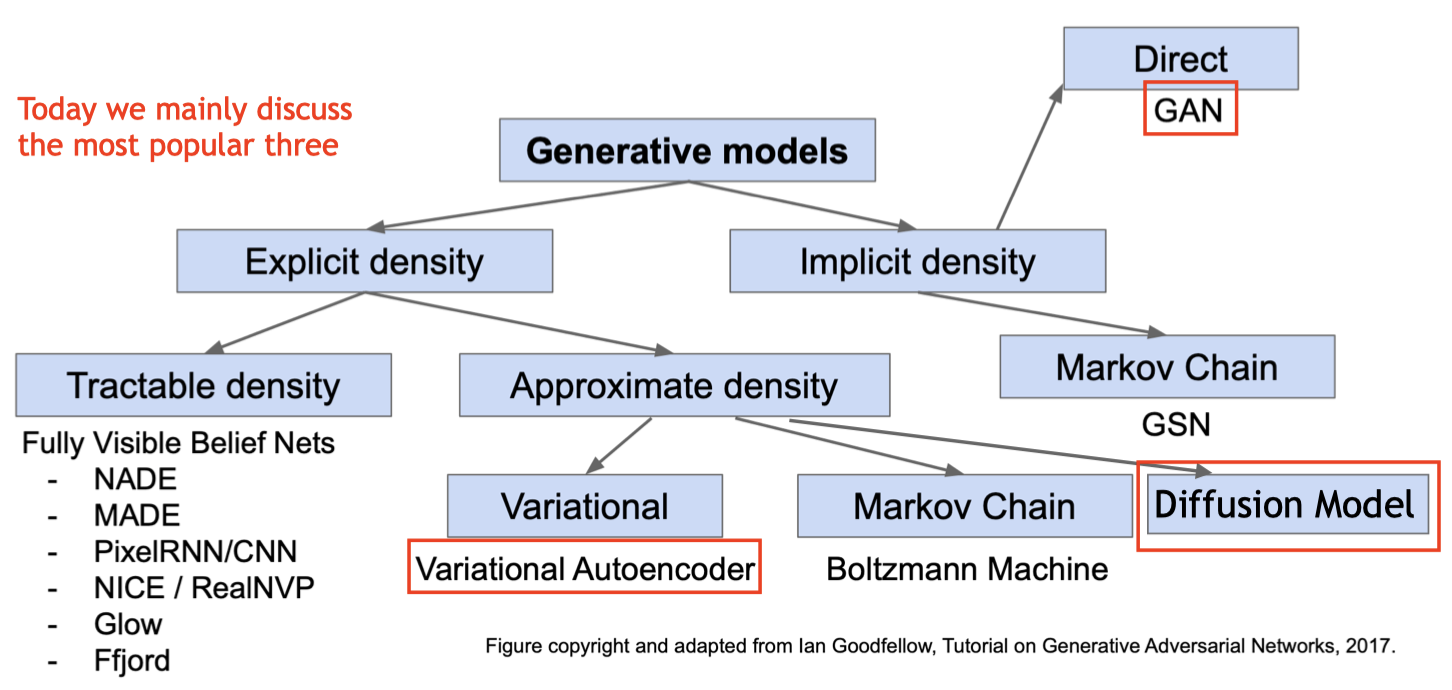
\includegraphics[scale=0.3]{figures/generative_model.png}
	\caption{生成模型分类}
	\label{fig:generative_model}
	\end{figure}

	如图\ref{fig:generative_model}所示,整体来讲有两种生成模型:隐式和显式.
	显式模型是expilcity density model, or Fully Visible Belief Network (FVBN), 
	可以告诉你$p_{model}(x)$;而隐式模型则只能采样,不能告诉你概率分布.
	
	本门课接触三个生成模型:VAE,GAN,Diffusion Model
	
	但是图中Tractable Density模型最容易理解,先说一下

	\subsection{Tractable Density Model}

	假设我们的隐式概率模型是$p(x) = p(x_1, \cdots, x_n)$,应用链式法则可得:
	
	\begin{equation}
		p(x)=\prod_{i=1}^{n} p\left(x_{i} \mid x_{1}, \ldots, x_{i-1}\right)
	\end{equation}
	
	什么样的神经网络能够处理这样的连续的条件概率?(显然我们希望获得一个shared网络)
	
	PixelRNN,PixelCNN
	
	优点:loss直观,容易优化,sample方便
	
	缺点:由于存在序列关系,所以慢,并且序列关系对于图片是没有意义的
	
	\subsection{VAE}

	看过很多生成模型的博客,这个博客是写的最好的:
	\href{https://lilianweng.github.io/posts/2018-08-12-vae/}
	{From Autoencoder to Beta-VAE}
	
	\begin{equation}
		p_{\theta}(x)=\int p(z) p_{\theta}(x \mid z) \mathrm{d}z
	\end{equation} 
	
	前面我们曾经讲过AutoEncoder的概念,其实它可以视为一种降维手段,
	将原数据通过一定处理(如多层神经网络)获得其另一种表示(或称编码),
	这个过程就是encode,然后需要时可以进行解码恢复.它本质上可以视为学习两个映射:

	\begin{equation}
		\begin{array}{l}
			\phi: \mathcal{X} \rightarrow \mathcal{F} \\
			\psi: \mathcal{F} \rightarrow \mathcal{X} \\
			\phi, \psi=\underset{\phi, \psi}{\arg \min }\|\mathcal{X}-(\psi \circ \phi) \mathcal{X}\|^{2}
		\end{array}
	\end{equation}

	看起来在前面的AE当中,我们只需要decoder部分就可以完成生成.
	实果真如此吗?如果只有decoder,那么z服从何种分布完全不了解(总不能是均匀分布吧).

	然后考虑这个模型的Loss:

	\begin{equation}
		p_\theta(x)=\int p(z)p_\theta(x|z)dz
	\end{equation}

	如何计算积分?
	积分里面的两项都容易算,但是其积分不容易计算.
	
	那么,Monte Carlo方法可以吗:
	
	\begin{equation}
		p_\theta(x)=\mathbf{E}_{z\sim p(z)}[p_\theta(x|z)]\\
		\log p(x) \approx \log \frac{1}{k} \sum_{i=1}^{k} p_{\theta}\left(x \mid z^{(i)}\right), \text { where } z^{(i)} \sim p(z)
	\end{equation}
	
	如果使用蒙特卡洛方法估计,维数太高,方差太高,需要sample太多了.

	直接计算不行, Monte Carlo不行,那么试试Bayes公式,
	如果能够引入后验概率$p_{\theta}(z|x)$:

	\begin{equation}
		p_{\theta}(x)=\frac{p_{\theta}(x, z)}{p_{\theta}(z \mid x)}=
		\frac{1}{p_{\theta}(z \mid x)} p(z) p_{\theta}(x \mid z)
	\end{equation}

	但是$p_{\theta}(z \mid x)$还没有,我们希望学一个神经网络近似
	$p_{\theta}(z \mid x)$,也就是学习一个$q_{\phi}(z|x)$
	来近似$p_{\theta}(z|x)$.

	变分自编码器的Variatinal就是指这个近似, 使得$q_{\phi}(z|x)$
	来近似$p_{\theta}(z|x)$.

	\textbf{
	注意对于VAE的基本假设有如下三条
	\begin{enumerate}
		\item $p(z)$已知,是一个高维标准正态分布
		\item $p_\theta(x|z)$函数族已知,一个均值和方差来源于神经网络的正态分布
		\item $q_\phi(z|x)$函数族已知,一个均值和方差来源于神经网络的正态分布
	\end{enumerate}
	当然$p (z)$是高维标准正态分布这个假设不是很合理,这也是VAE的一个limitation,但是在一定程度上是可以接受的}
	
	\textbf{再次 Formulate 一下这个工作:}
	
	假设所有已知数据$\bm x$来自一个未知的概率分布$P(\bm x)$,
	我们希望用一组参数$\theta$来确定一个参数分布$p_{\theta}(\bm x)$来拟合
	$P(\bm x)$.我们假定$\bm x$与另一些隐变量$\bm z$有关,那么依据边缘分布和条件分布
	的相关性质可知
	\begin{equation}
		p_{\theta}(\bm x) = \int_{\bm z} p_\theta(\bm x, \bm z) \dd \bm z = \int_{\bm z} p_\theta(\bm x\mid \bm z) p_{\theta}(\bm z) \dd \bm z
	\end{equation}

	这里$p(\bm z)$一般被称为先验分布,一般取其为标准正态分布\marginpar{\kaishu 
	正因为$\bm z$是先验的,所以$p_{\theta}(\bm z)$也可以写成$p(\bm z)$,
	因为它没有参数.}.而$p_{\theta}(\bm z \mid \bm x)$则被称为后验分布.
	编码器学习的就是$p_{\theta}(\bm z \mid \bm x)$, 因为它代表了如何从
	$\bm x$转换到隐变量.解码器学习的则是$p_{\theta}(\bm x \mid \bm z)$.
	
	上式并不能解决我们的问题.尽管我们确定了先验分布,而且
	$p_{\theta}(\bm x \mid \bm z)$可由解码器学习,但上式的积分是难以计算的,
	因为实际操作中我们不可能遍历$\bm z$所在的高维空间.所以我们试图用贝叶斯公式曲线救国:
	
	\begin{equation}
		p_{\theta}(\bm x) = \frac{p_\theta(\bm x\mid \bm z) p(\bm z)}{p_\theta(\bm z\mid \bm x)}
	\end{equation}

	那么$p_\theta(\bm z\mid \bm x)$又怎么获得呢?这其实是编码器负责学习的分布,
	\marginpar{\kaishu 这可能就是神经网络之道:凡是不容易算不好表示的东西,
	通通丢给神经网络去学习...}因此我们用编码器来学习它.
	我们记编码器学习的分布为$q_\phi(\bm z\mid \bm x)$.
	
	那么如何度量学习的好坏呢?我们知道两个分布的差异可以用KL-divergence度量.
	
	最后我们用一句话来概括VAE的工作,然后进入形式化的推导:在VAE当中,
	输入数据$\bm X$是来自于一个特定的先验参数分布$p_{\theta}(\bm x)$,
	随后我们同时训练encoder和decoder,使得在我们学习的后验分布
	$q_\phi(\bm z\mid \bm x)$和真实后验分布$p_\theta(\bm z\mid \bm x)$
	的KL散度$\operatorname{D_{KL}}(q_\phi \parallel p_\theta)$
	作为度量之下的重建误差最小.

	\textbf{接下来推导Loss:}
	
	计算学习的后验分布$q_\phi(\bm z\mid \bm x)$和真实后验分布
	$p_\theta(\bm z\mid \bm x)$的KL散度
	$\operatorname{D_{KL}}(q_\phi \parallel p_\theta)$得到:
	\begin{equation}
		\begin{aligned}
			\operatorname{D_{KL}}\left(q_{\phi}(\bm{z} \mid \bm{x}) \| p_{\theta}(\bm{z} \mid \bm{x})\right) &=\int q_{\phi}(\bm{z} \mid \bm{x}) \log \frac{q_{\phi}(\bm{z} \mid \bm{x})}{p_{\theta}(\bm{z} \mid \bm{x})} \dd \bm{z} \\
			&=\int q_{\phi}(\bm{z} \mid \bm{x}) \log \frac{q_{\phi}(\bm{z} \mid \bm{x}) p_{\theta}(\bm{x})}{p_{\theta}(\bm{z}, \bm{x})} \dd \bm{z} \\
			&=\int q_{\phi}(\bm{z} \mid \bm{x})\left(\log \left(p_{\theta}(\bm{x})\right)+\log \frac{q_{\phi}(\bm{z} \mid \bm{x})}{p_{\theta}(\bm{z}, \bm{x})}\right) \dd \bm{z} \\
			&=\log \left(p_{\theta}(\bm{x})\right)+\int q_{\phi}(\bm{z} \mid \bm{x}) \log \frac{q_{\phi}(\bm{z} \mid \bm{x})}{p_{\theta}(\bm{z}, \bm{x})} \dd \bm{z} \\
			&=\log \left(p_{\theta}(\bm{x})\right)+\int q_{\phi}(\bm{z} \mid \bm{x}) \log \frac{q_{\phi}(\bm{z} \mid \bm{x})}{p_{\theta}(\bm{x} \mid \dd \bm{z}) p_{\theta}(\bm{z})} \dd \bm{z} \\
			&=\log \left(p_{\theta}(\bm{x})\right)+E_{\bm{z} \sim q_{\phi}(\bm{z} \mid \bm{x})}\left(\log \frac{q_{\phi}(\bm{z} \mid \bm{x})}{p_{\theta}(\bm{z})}-\log \left(p_{\theta}(\bm{x} \mid  \bm{z})\right)\right) \\
			&=\log \left(p_{\theta}(\bm{x})\right)+\operatorname{D_{KL}}\left(q_{\phi}(\bm{z} \mid \bm{x}) \| p_{\theta}(\bm{z})\right)-\mathbb E_{\bm{z} \sim q_{\phi}(\bm{z} \mid \bm{x})}\left(\log \left(p_{\theta}(\bm{x} \mid \bm{z})\right)\right)
		\end{aligned}
	\end{equation}
	
	将上式重写成
	\begin{equation}
		\log \left(p_{\theta}(\bm{x})\right) - \operatorname{D_{KL}}\left(q_{\phi}(\bm{z} \mid \bm{x}) \| p_{\theta}(\bm{z} \mid \bm{x})\right) = -\operatorname{D_{KL}}\left(q_{\phi}(\bm{z} \mid \bm{x}) \| p_{\theta}(\bm{z})\right)+\mathbb E_{\bm{z} \sim q_{\phi}(\bm{z} \mid \bm{x})}\left(\log \left(p_{\theta}(\bm{x} \mid \bm{z})\right)\right)
	\end{equation}
	
	左侧第一项是我们希望最大化的输出的概率,第二项是希望最小化的分布差异,
	综合起来应该最大化左侧.我们再来看右侧,第一项是$q_{\phi}(\bm{z} \mid \bm{x})$
	和$p(\bm z)$之间的KL散度,最小化这一项说明我们希望后验分布也符合正态.
	最后一项最大化则是希望我们的解码器预测更加准确.使用优化理论的常用手段,
	我们将损失函数定义为
	\begin{equation}
		\mathcal{L}_{\theta, \phi} = -RHS = \operatorname{D_{KL}}\left(q_{\phi}(\bm{z} \mid \bm{x}) \| p_{\theta}(\bm{z})\right)-\mathbb E_{\bm{z} \sim q_{\phi}(\bm{z} \mid \bm{x})}\left(\log \left(p_{\theta}(\bm{x} \mid \bm{z})\right)\right)
	\end{equation}

	我们希望求得
	\begin{equation}
		\theta^{*}, \phi^{*} = \arg\min_{\theta, \phi} \mathcal{L}_{\theta, \phi}
	\end{equation}

	\begin{figure}[htbp]
		\centering
		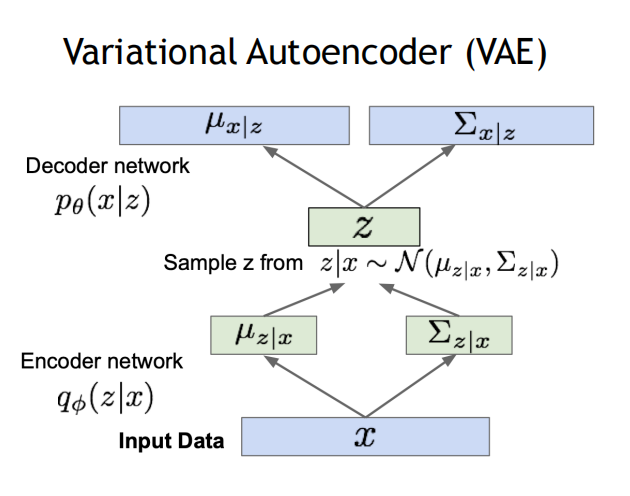
\includegraphics[scale=0.5]{figures/VAE_2.png}
		\caption{VAE结构}
		\label{fig:VAE_structure}
	\end{figure}

	我们的网络结构如图\ref{fig:VAE_structure}所示,它由两部分组成.

	现在我们来看看这两项具体如何运算.
	
	第一项,由于我们假定后验分布也是高斯分布,
	两个高斯分布的KL散度有Closed form solution\marginpar{\kaishu 
	因为我们假定后验分布的隐变量彼此独立,即
	$\bm \Sigma = \diag \{ \sigma_1^2, \cdots, \sigma_d^2\}$, 
	因此多维的情形可以由一维计算后求和.计算过程略.}

	虽然我们添加这一项希望其接近高斯,
	但这一项绝不可真正为0,否则就与x无关了,这样就不含x的信息了,从而不可能进行重建.
	
	\begin{equation}
		\operatorname{D_{KL}}(p(\bm z \mid \bm x) \| q(\bm z))=\frac{1}{2} \sum_{k=1}^{d}\left(\mu_{(k)}^{2}(x)+\sigma_{(k)}^{2}(x)-\ln \sigma_{(k)}^{2}(x)-1\right)
	\end{equation}
	
	对于后验分布,我们有
	\begin{equation}
		q(\bm x \mid \bm z)=\frac{1}{\prod_{k=1}^{D} \sqrt{2 \pi \tilde{\sigma}_{(k)}^{2}(\bm z)}} \exp \left(-\frac{1}{2}\left\|\frac{\bm x-\tilde{\mu}(\bm z)}{\tilde{\sigma}(\bm z)}\right\|^{2}\right)
	\end{equation}

	得到
	\begin{equation}
		-\ln q(\bm x \mid \bm z)=\frac{1}{2}\left\|\frac{\bm x-\tilde{\mu}(\bm z)}{\tilde{\sigma}(\bm z)}\right\|^{2}+\frac{D}{2} \ln 2 \pi+\frac{1}{2} \sum_{k=1}^{D} \ln \tilde{\sigma}_{(k)}^{2}(\bm z)
	\end{equation}

	\begin{figure}[htbp]
		\centering
		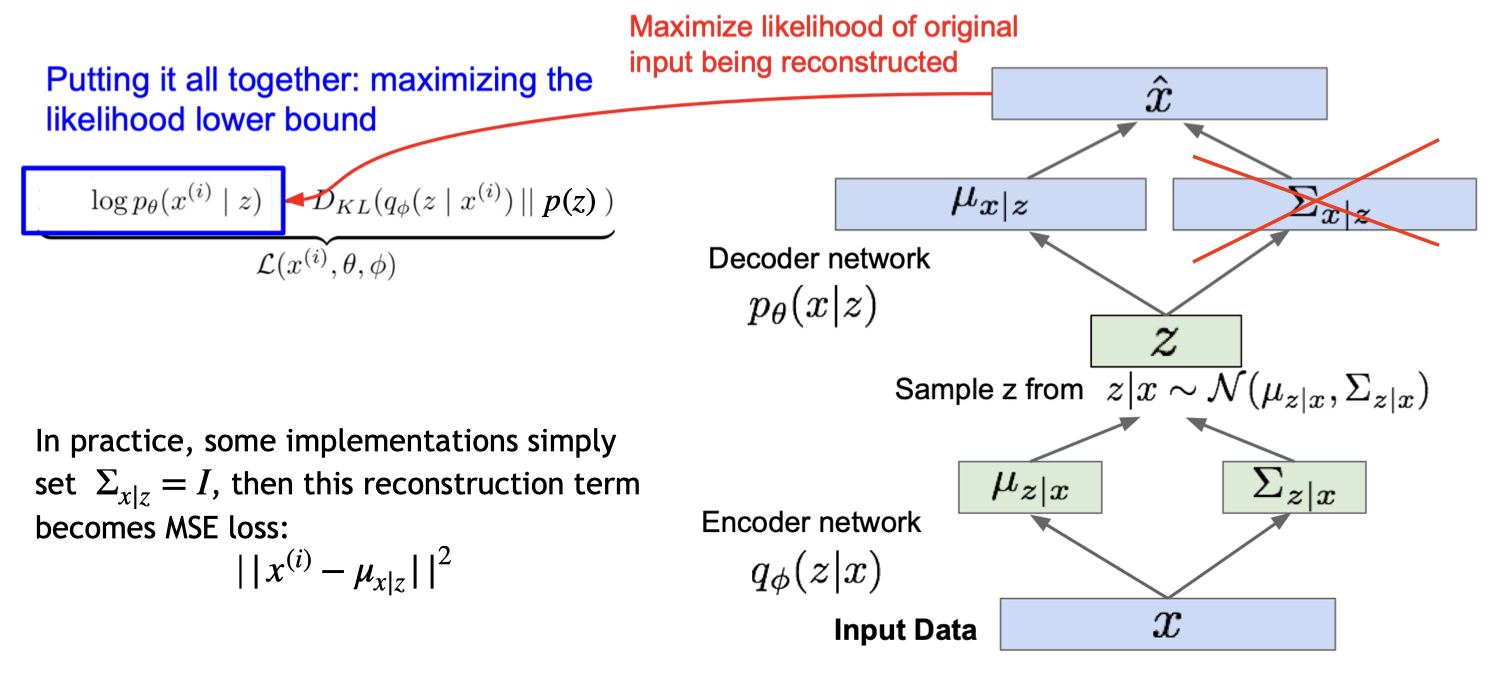
\includegraphics[scale=0.3]{figures/simple_VAE.png}
		\caption{简化的 VAE 结构}
		\label{fig:simple_VAE}
	\end{figure}

	第二项,也就是让网络输出的分布的接近真实的分布
	(注意上式的$x$并不是网络输出,而是输入)
	
	因此,VAE的loss非常有趣,它的$\phi$看似只出现在第一项,但实际上还出现在第二项的$z$
	里面,因此我们将$z$写成$z=\mu_{z \mid x}+\epsilon \sigma_{z \mid x}$,
	从而有梯度可以回传.另外,ELBO的计算也是intractable的,因为第一项的
	$\mathbb{E}_{z}$这一步就计算不出来,我们直接扔掉期望,取它自己作为Monte Carlo的估计.
	
	这里和最开始说Monte Carlo的地方相比较,
	两个被估计的量分别是$\log\xk{\mathbb{E}_z \zk{p_{\theta} \xk{x^{(i)}  \mid z}}}$
	和$\mathbb{E}_{z} \log p_{\theta} \xk{x^{(i)}\mid z}$,
	前者的$z \sim p$,后者则是$q$,后者实际上更加集中,方差更小.
	
	实际上我们有时直接令$\Sigma_{x \mid z} = \bd I$.因为loss当中,形式为

	\begin{equation}
		\exp^{-\xk{\frac{x - \mu}{\sigma}}^2}
	\end{equation}

	所以如图\ref{fig:simple_VAE}所示,我们可以将VAE简化为一个简单的网络结构:
	令decoder的$\sigma = 1$,即协方差矩阵为单位阵.否则对于上面这一项,
	网络可以通过一直增大方差的方式来减小loss,如果$\sigma = 1$,
	损失函数就没有了分母,变为MSE.

	\textbf{为什么使用高斯分布?}
	
	\begin{enumerate}
		\item 高斯分布简单,可以通过均值和方差完全描述
		\item 高斯分布的KL散度有解析解, 满足线性性, 可以进行缩放方便地进行重参数化
		\item 高斯分布的采样很容易
	\end{enumerate}
	
	\textbf{这东西跟变分 (variational)究竟有什么关系?}
	
	要说起变分,先讲泛函.泛函简单地说就是函数的函数,或广义的函数.

	变分,是指自变量\textbf{函数}发生的变化,为与自变量的变化$\dd x$区分,
	我们一般用$\delta$表示.例如我们想要求解空间中$A, B$两点之间最短的曲线,
	设任意一条曲线为$f(x, y)$,其长度为

	\begin{equation}
		l = \int_{A}^{B} f(x,  y) \dd s.
	\end{equation}

	当自变量函数$f$发生微小变化$\delta f$时,长度也发生了$\delta l$的变化.
	运用EL方程,我们可以求得$\frac{\delta l}{\delta f} = 0$
	时的函数$f$.
	
	在VAE当中,我们实际上也是希望找到$q_\theta$来近似$p_{\theta}$,
	这是在说两个函数之间的距离很小;
	这就类似于变分的时候找一个函数去逼近最速降线,
	使得降落时间不变,也是在考虑两个函数之间的距离.

	但是实际上我们并没有使用任何变分法的技术,因为变分法是不知道连续性之外任何函数的先验知识的,
	但是这里对于神经网络我们已经加入了神经网络进行参数化,从而将搜索空间限制为神经网络的参数空间上,
	而非更高阶无限维的函数空间.

	现在提到变分 (Variational),都是引入了ELBO进行近似的.

	\subsection{GAN}

	有了GAN,不代表VAE没用了,在不要求清晰度的情况下,VAE还是有很大发挥空间的.
	
	\begin{equation}
		\min _{\theta_{g}} \max _{\theta_{d}}\left[\mathbb{E}_{x \sim p_{d a t a}} \log D_{\theta_{d}}(x)+\mathbb{E}_{z \sim p(z)} \log \left(1-D_{\theta_{d}}\left(G_{\theta_{g}}(z)\right)\right)\right]
	\end{equation}

	交替训练.防止梯度相似?
	
	\marginpar{discriminator: 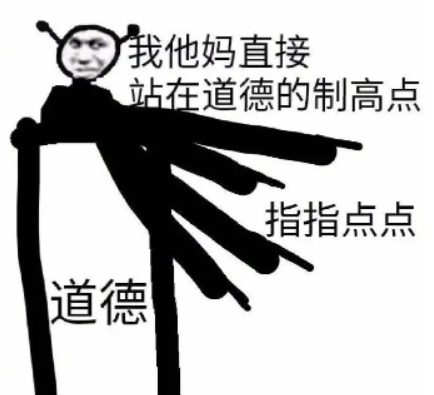
\includegraphics[scale=0.25]{figures/ddgg.png}}
	
	但是有一点值得注意:上式中$\log(1-x)$这一函数在$x$接近$0$时梯度非常小.
	而训练之初,discriminator可以轻易辨别出generator生成的图片为假,
	而generator的梯度又太小,于是就形成了discriminator把generator按在墙角使劲打,
	后者还跑不出去(笑).
	
	总之,这个loss对于generator是很不利的.所以可以改变一下loss的形式.
	
	\textbf{Non-Saturating Loss functions}
	
	Gradient ascent on discriminator:
	
	\begin{equation}
	\max_{\theta_d}\left[\mathbb{E}_{x\sim p_{data}}\log D_{\theta_d}(x)+\mathbb{E}_{z\sim p(z)}\log(1-D_{\theta_d}(G_{\theta_g}(z)))\right]
	\end{equation}

	Gradient descent on generator:

	\begin{equation}
	\min_{\theta_g}\mathbb{E}_{z\sim p(z)}\log(1-D_{\theta_d}(G_{\theta_g}(z)))	
	\end{equation}

	\textbf{\\为什么每一个 iteration 多次训练 Discriminator 但是只训练一次 Generator?}

	因为训练 Generator 的时候梯度要流过 Discriminator,如果 Discriminator 训练的次数太少,
	Discriminator 找到的错误就不对, 因此 Generator 的梯度也不对, 会导致训练不稳定.

	所以一个好老师很重要.

	\textbf{\\GAN在单一分布上效果很好,但是在大规模数据集很差,为什么?}

	Mode chasing → Mode collapse: 生成器一直选择和输入一样的图片输出,
	辨别器一直说这是假的,最后导致生成器生成的图片都是同样的,这就是模式崩塌.

	VAE要求所有类型都为真,而GAN则只需要保证"我生成的"图片真.
	
	这个问题最后也没解决.

	\textbf{\\Metrics}

	如何衡量网络的表现?很难有客观的度量.
	
	1.最近邻: 检测过拟合,生成的样本和训练集中其最近邻进行对比

	2.用户研究: 参与者被要求在短时间内(例如100毫秒)区分生成的样
	本和真实图像或者根据生成图像的逼真度对模型进行排名 

	3.模式丢失和模式崩溃: 对于具有已知模式的数据集通过测
	量生成数据到模式中心的距离来计算模式大小
	
	这也是我们之前interpolation要求渐变的原因,防止你只学了个记忆功能.
	如果是这样,那么连续变化会有非常明显的不连续.
	
	有没有定量的 GAN Generator Evaluation?

	Quantitative Measurement: FID
	
	FID实际上就是将gt和生成图片都转换到一个特征空间,随后认为其符合正态,度量其统计参数.
	
	\begin{equation}
		\operatorname{FID}(r, g)=\left\|\mu_{r}-\mu_{g}\right\|_{2}^{2}+\operatorname{Tr}\left(\Sigma_{r}+\Sigma_{g}-2\left(\Sigma_{r} \Sigma_{g}\right)^{\frac{1}{2}}\right)
	\end{equation}

	\begin{figure}[htbp]
		\centering
		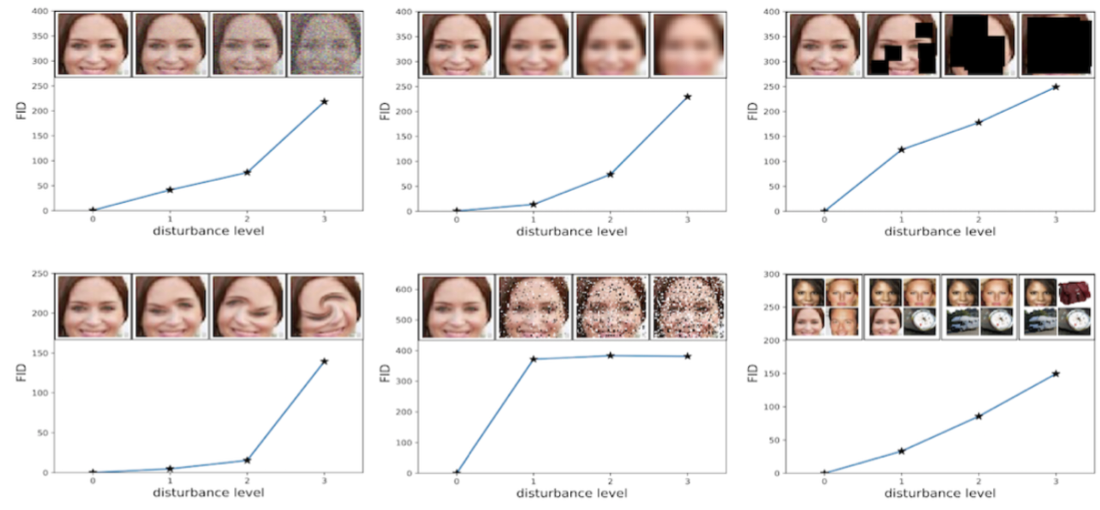
\includegraphics[scale=0.3]{figures/fid.png}
		\caption{image distortions 对FID 的影响}
		\label{fig:fid}
	\end{figure}

	如图\ref{fig:fid}所示,FID measure 对图像失真敏感。
	从左上到右下:高斯噪声、高斯模糊、植入的黑色矩形、
	旋转图像、salt and pepper 噪声,以及被ImageNet图像污染的CelebA数据集。
	
	GAN在语义上的加减:生成好的图片的网络,其隐变量也必然学习了一些好的特征.latent
	space structure有一定的线性代数结构.
	
	\subsection{Diffusion Model}

	不会考很深.

	本质就是解决VAE的latent space是固定的标准正态分布的问题.

	向大家推荐这个博客:\href{https://lilianweng.github.io/posts/2021-07-11-diffusion-models/}{What are Diffusion Models?}.
